\documentclass[a4paper, 11pt]{article}
\usepackage{hyperref}
\hypersetup{
    colorlinks=true,
    linkcolor=blue,
    filecolor=red,      
    urlcolor=red,
    pdftitle={Overleaf Example},
    pdfpagemode=FullScreen,
    }
\usepackage{graphicx,wrapfig,subfigure,amsmath,amssymb,epsfig,bm}
\usepackage{listings,textcomp,color,geometry}
\geometry{hmargin=2cm, vmargin=2cm}
\usepackage[dvipsnames]{xcolor}
\usepackage{amsmath}
\usepackage{tikz}
\usepackage{listings}

\lstset{language=Python, 
        basicstyle=\ttfamily\small, 
        keywordstyle=\color{blue},
        stringstyle=\color{red},
        commentstyle=\color{red},
        frame=single,
        breaklines=true,
        numbers=left,
        numberstyle=\tiny\color{gray},
        stepnumber=1,
        tabsize=4}



\def\Box{\mathord{\dalemb{7.9}{8}\hbox{\hskip1pt}}}
\def\dalemb#1#2{{\vbox{\hrule height.#2pt
        \hbox{\vrule width.#2pt height#1pt \kern#1pt \vrule width.#2pt}
        \hrule height.#2pt}}}

\def\eop{\mathcal{E}}
\def\bop{\mathcal{B}}
\def\ba{\begin{eqnarray}}
\def\ea{\end{eqnarray}}
\def\be{\begin{equation}}
\def\ee{\end{equation}}
\def\tr{{\rm tr}}
\def\Var{{\rm Var}}
\def\gtorder{\mathrel{\raise.3ex\hbox{$>$}\mkern-14mu
             \lower0.6ex\hbox{$\sim$}}}
\def\ltorder{\mathrel{\raise.3ex\hbox{$<$}\mkern-14mu
             \lower0.6ex\hbox{$\sim$}}}

\def\bb{{\mathfrak b}}
\newcommand{\ellb }{\boldsymbol{\ell }}

\definecolor{denim}{rgb}{0.08, 0.38, 0.74}
\definecolor{ao}{rgb}{0.0, 0.5, 0.0}

% Personal colors defined here
\newcommand{\red}[1]{{\color{red}#1}}
\newcommand{\green}[1]{{\color{ForestGreen}#1}}
\newcommand{\cyan}[1]{{\color{Orange}#1}}
\newcommand{\blue}[1]{{\color{denim}#1}}
\newcommand{\assume}[1]{{\bf#1}}

\title{The ACT measurement of the lensing power spectrum}

\begin{document}

\maketitle

In April 2023, the Atacama Cosmology Telescope collaboration has released a measurement of a \href{https://arxiv.org/abs/2304.05203}{signal dominated lensing map} over a quarter of the sky, and its \href{https://arxiv.org/abs/2304.05202}{associated power spectrum}. The goal of this tutorial is to compute 
the underlying theoretical lensing power spectrum in the $\Lambda$CDM model and compare it to the data.

\begin{figure}[h!]
  \centering
  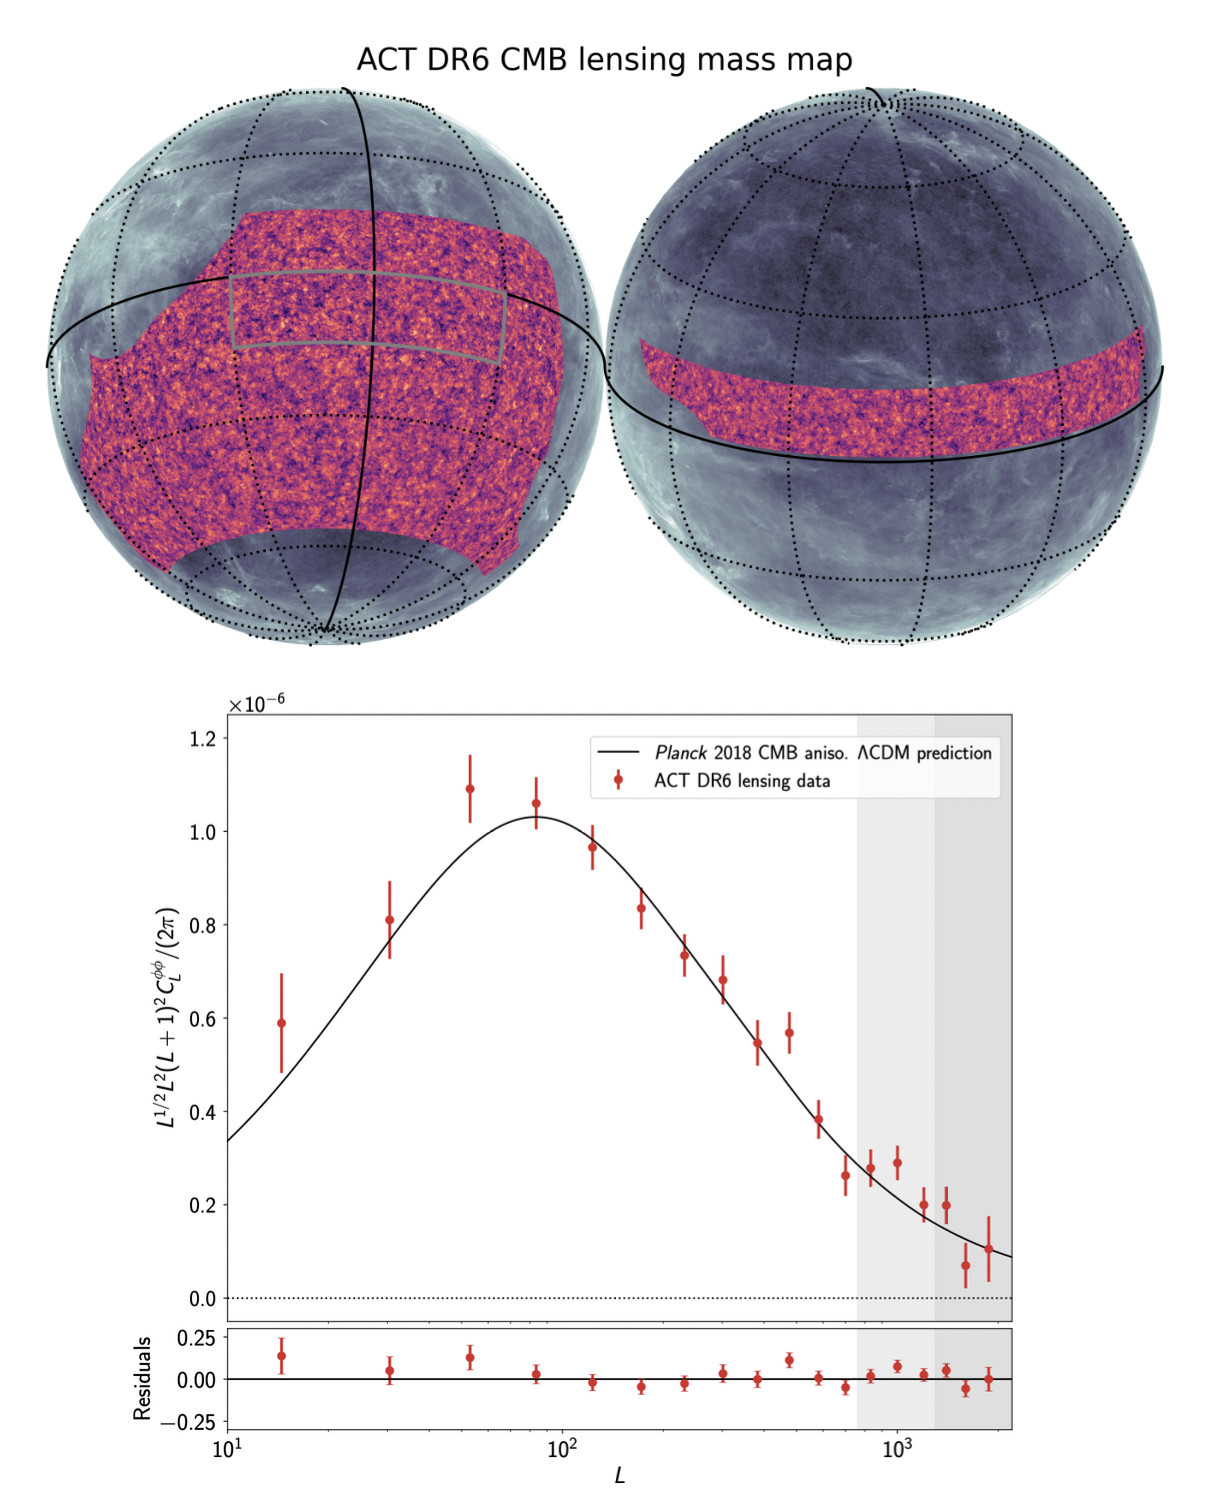
\includegraphics[width=0.7\columnwidth]{lensing_dr6.png}
  \caption{Top: ACT DR6 CMB lensing mass map presented in this work. The map covers 9400 ${\rm deg}^{2}$
or sky fraction $f_{\rm sky} = 0.23$ with a signal-to-noise significantly greater than unity over a wide range of scales. Bright orange corresponding to peaks of the dark-matter dominated mass distribution and
dark purple regions corresponding to voids. Bottom: the ACT DR6 lensing potential power spectrum bandpowers for our baseline (combined temperature and polarization) analysis}
  \label{fig:dr6_lensing}
\end{figure}



Useful quantities
\ba
1 \ \rm{Mpc} &=& 3.086 \times 10^{22} \ m \nonumber \\
G &=& 6.674 \times 10^{-11}  \  m^{3} kg^{-1} s^{-2} \nonumber \\
m_{H} &=& 1.6735575  \times10^{-27}  \ kg\nonumber \\
c &=& 3 \times 10^{8} \ m s^{-1} \nonumber \\
\ea


\section{Energy densities}


{\it The first step to compute the prediction for the form and amplitude of the $\Lambda$CDM lensing power spectrum is to compute the density of the different components in the Universe.}  \\

We will work in the LCDM framework with the following cosmological parameters:
\ba
T_{\rm CMB} &=& 2.7255 \  \rm{K} \nonumber \\
H_{0} &=& 67.5 \ \rm{ km/s/Mpc} \nonumber   \\
\Omega_{\rm b}h^{2} &=& 0.022 \nonumber   \\
\Omega_{\rm cdm}h^{2} &=& 0.122  \nonumber \\
\Omega_{\rm m} &=&  \Omega_{\rm b} +  \Omega_{\rm cdm}
\ea


$\Omega_{b}$ stands for Omega baryons, and is defined as the ratio of the current baryon density  over the current critical density of the Universe 
\ba
\Omega_{b} = \frac{\rho^{0}_{b}}{\rho^{0}_{c}}  \nonumber
\ea
the critical density today is defined such as
\ba
\rho^{0}_{c} = \frac{3H^{2}_{0}}{8\pi G}
\ea 
and $h$ is the reduced Hubble factor 
\ba
h = \frac{H_{0}}{100}
\ea
\begin{enumerate}
\item Compute numerically the value of $H_{0}$ in $s^{-1}$ unit.
\item Compute numerically the value of $\rho^{0}_{b}$ and $\rho^{0}_{\rm cdm}$ in $\rm{kg}/m^{3}$, let's assume that all baryonic matter is composed of hydrogen, how many hydrogen atoms is there per cubic meter in the universe ?
\item Photons at equilibrium with temperature $T_{\rm CMB}$ follow a Bose-Einstein distribution $f_{\gamma}(\nu | T_{\rm CMB}) = \left[\exp \left(\frac{h\nu}{k_{B}T_{CMB}} \right)-1\right]^{-1}$, the energy density of photons is given by
\ba
\rho^{0}_{\gamma} c^{2}= 2 \int \frac{d^{3}p}{(2\pi \hbar)^{3}} h\nu f_{\gamma}(\nu | T_{\rm CMB}) 
\ea
for photons, $p = \frac{h\nu}{ c}$, setting $x = \frac{h\nu}{k_{B}T_{\rm CMB}}$ show that the integral can be written
\ba
\rho^{0}_{\gamma} c^{2}= \frac{ (k_{B}T_{\rm CMB})^{4}}{\hbar^{3}c^{3}\pi^{2}} \int dx x^{3}  \left[\exp \left(x)-1\right)\right]^{-1}
\ea
Using $\Gamma(s) \zeta(s)  = \int_{0}^{\infty} \frac{t^{s-1}}{e^{t}-1}dt$
and  $\Gamma(4) = 3!$, $\zeta(4) = \frac{\pi^{4}}{90}$
Show that
\ba
\rho^{0}_{\gamma}  =  \frac{\pi^{2} (k_{B}T_{\rm CMB})^{4}}{15 \hbar^{3}c^{5}}
\ea
\item Compute $\Omega_{\gamma}$  numerically.
\item We also need to include the contribution from neutrinos, the formula for the neutrinos density is similar to the one of photons with some corrections, a factor $\frac{7}{8}$ coming from the fact that neutrinos are fermions and a factor $(4/11)^{4/3}$ coming from the fact that neutrinos are a bit colder than photons because they decouple before the electron-positron annihilation (which reheat the plasma) $T_{\nu} = (4/11)^{1/3} T_{\gamma}$, we also need to account for the fact that there are three species of neutrinos $N_{\rm eff} =3.046$ (the fact that it is not exactly 3 comes from QED correction)
\ba
\rho^{0}_{\nu}  =  N_{\rm eff}  \frac{7}{8} \frac{\pi^{2} (k_{B}T_{\nu})^{4}}{15 \hbar^{3}c^{5}} = N_{\rm eff}  \frac{7}{8}  (4/11)^{4/3} \rho^{0}_{\gamma}
\ea
Compute $\Omega_{\rm rad} = \Omega_{\gamma} + \Omega_{\nu}$ numerically.
\item Get the value of $\Omega_{\Lambda}$ assuming that  $\Omega_{\rm m} + \Omega_{\rm rad} + \Omega_{\Lambda} = 1$, note that this relation is only true if the universe is flat (which is one of our assumptions here).  

\end{enumerate}

\begin{figure}
  \centering
  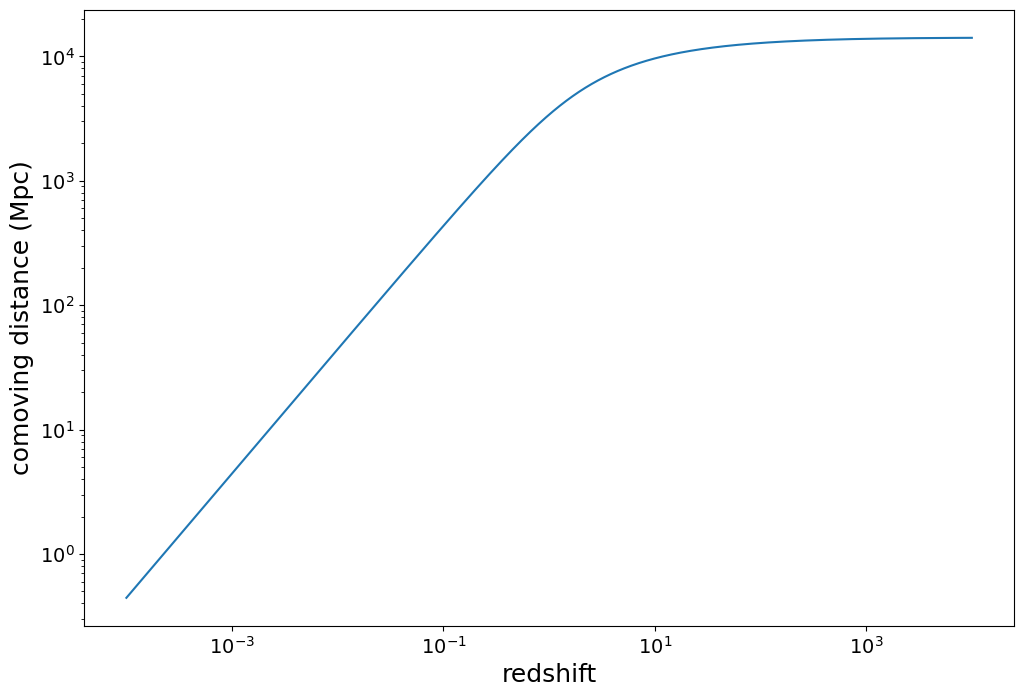
\includegraphics[width=0.7\columnwidth]{comoving_distance.png}
  \caption{comoving distance as a function of redshift in the LCDM Universe.}
  \label{fig:comov}
\end{figure}


\section{Distances}

{\it We will also need to be able to compute distance in the FLRW Universe}  \\

They are lot of useful distances definition in an expanding Universe, here we will use comoving distance. Imagine a pair of galaxies, their physical distance will increase due to the expansion of the Universe, but their comoving distance, which is measured with coordinates following the expansion of the Universe will stay fixed.
The comoving distance between us and an object at redshift z can be computed as  (see paragraph 1 of \href{https://github.com/thibautlouis/thibautlouis.github.io/blob/master/derivation.pdf}{notes})
\ba
\chi  = \int^{z}_{0}  \frac{c dz'}{ H(z')} \label{eq:confdistance}
\ea
Where 
\ba
H(z) = H_{0} \sqrt{ \Omega_{\rm rad}(1+z)^{4} + \Omega_{\rm m}(1+z)^{3} + \Omega_{\Lambda}} 
\ea
\begin{enumerate}
\item Compute numerically the co-moving distance between us and the last scattering surface, assuming the CMB is emitted at $z_{*}=1100$ and give its value in Mpc. What is its value in Giga light-year?, compare it to the age of the Universe which is $13.787$ Giga year.
\item Compute the comoving distance for an array of $10^{4}$ redshifts, logarithmically spaced\footnote{You can form the redshift array using np.logspace(-4,4,10000)}  between $z_{\rm min}=10^{-4}$ and $z_{\rm max}=10^{4}$, you should get something looking like Fig \ref{fig:comov}. 
 \item Something that will be useful for later is a way to get the redshift associated to a given comoving distance, so basically inverting Eq \ref{eq:confdistance}. A simple way to create this is to interpolate the array created in the previous question to get $z(\chi)$. you can use the python function: \\ \\
 
 \begin{lstlisting}[language=Python]
import numpy as np
from scipy.interpolate import InterpolatedUnivariateSpline

def interpolate_z_and_chi(H0, Omega_r, Omega_m, Omega_Lambda, logmin_z=-4, logmax_z=4, nz=10**4):

    """
    This function return the interpolation of z(chi)
    
    Parameters
     ----------
    H0: float
        Hubble constant value in km/s/Mpc
    Omega_r: float
        Omega radiation
    Omega_m: float
        Omega matter
    Omega_lambda: float
        Omega dark energy
    logmin_z: float
        Minimal value of log(z) for the interpolation
    logmax_z: float
        Maximum value of log(z) for the interpolation
    nz: integer
        number of z values
    """

    redshift = np.logspace(logmin_z, logmax_z, nz)
    chi  = np.zeros(nz)
    for i, z in enumerate(redshift):
        chi[i] = comoving_distance(z, H0, Omega_r, Omega_m, Omega_Lambda)
    z_of_chi = InterpolatedUnivariateSpline(chi, redshift)

    return z_of_chi

\end{lstlisting}

What is the redshift corresponding to a comoving distance of 1 Gpc ?
\end{enumerate}


\section{Lensing}

\begin{figure}
  \centering
  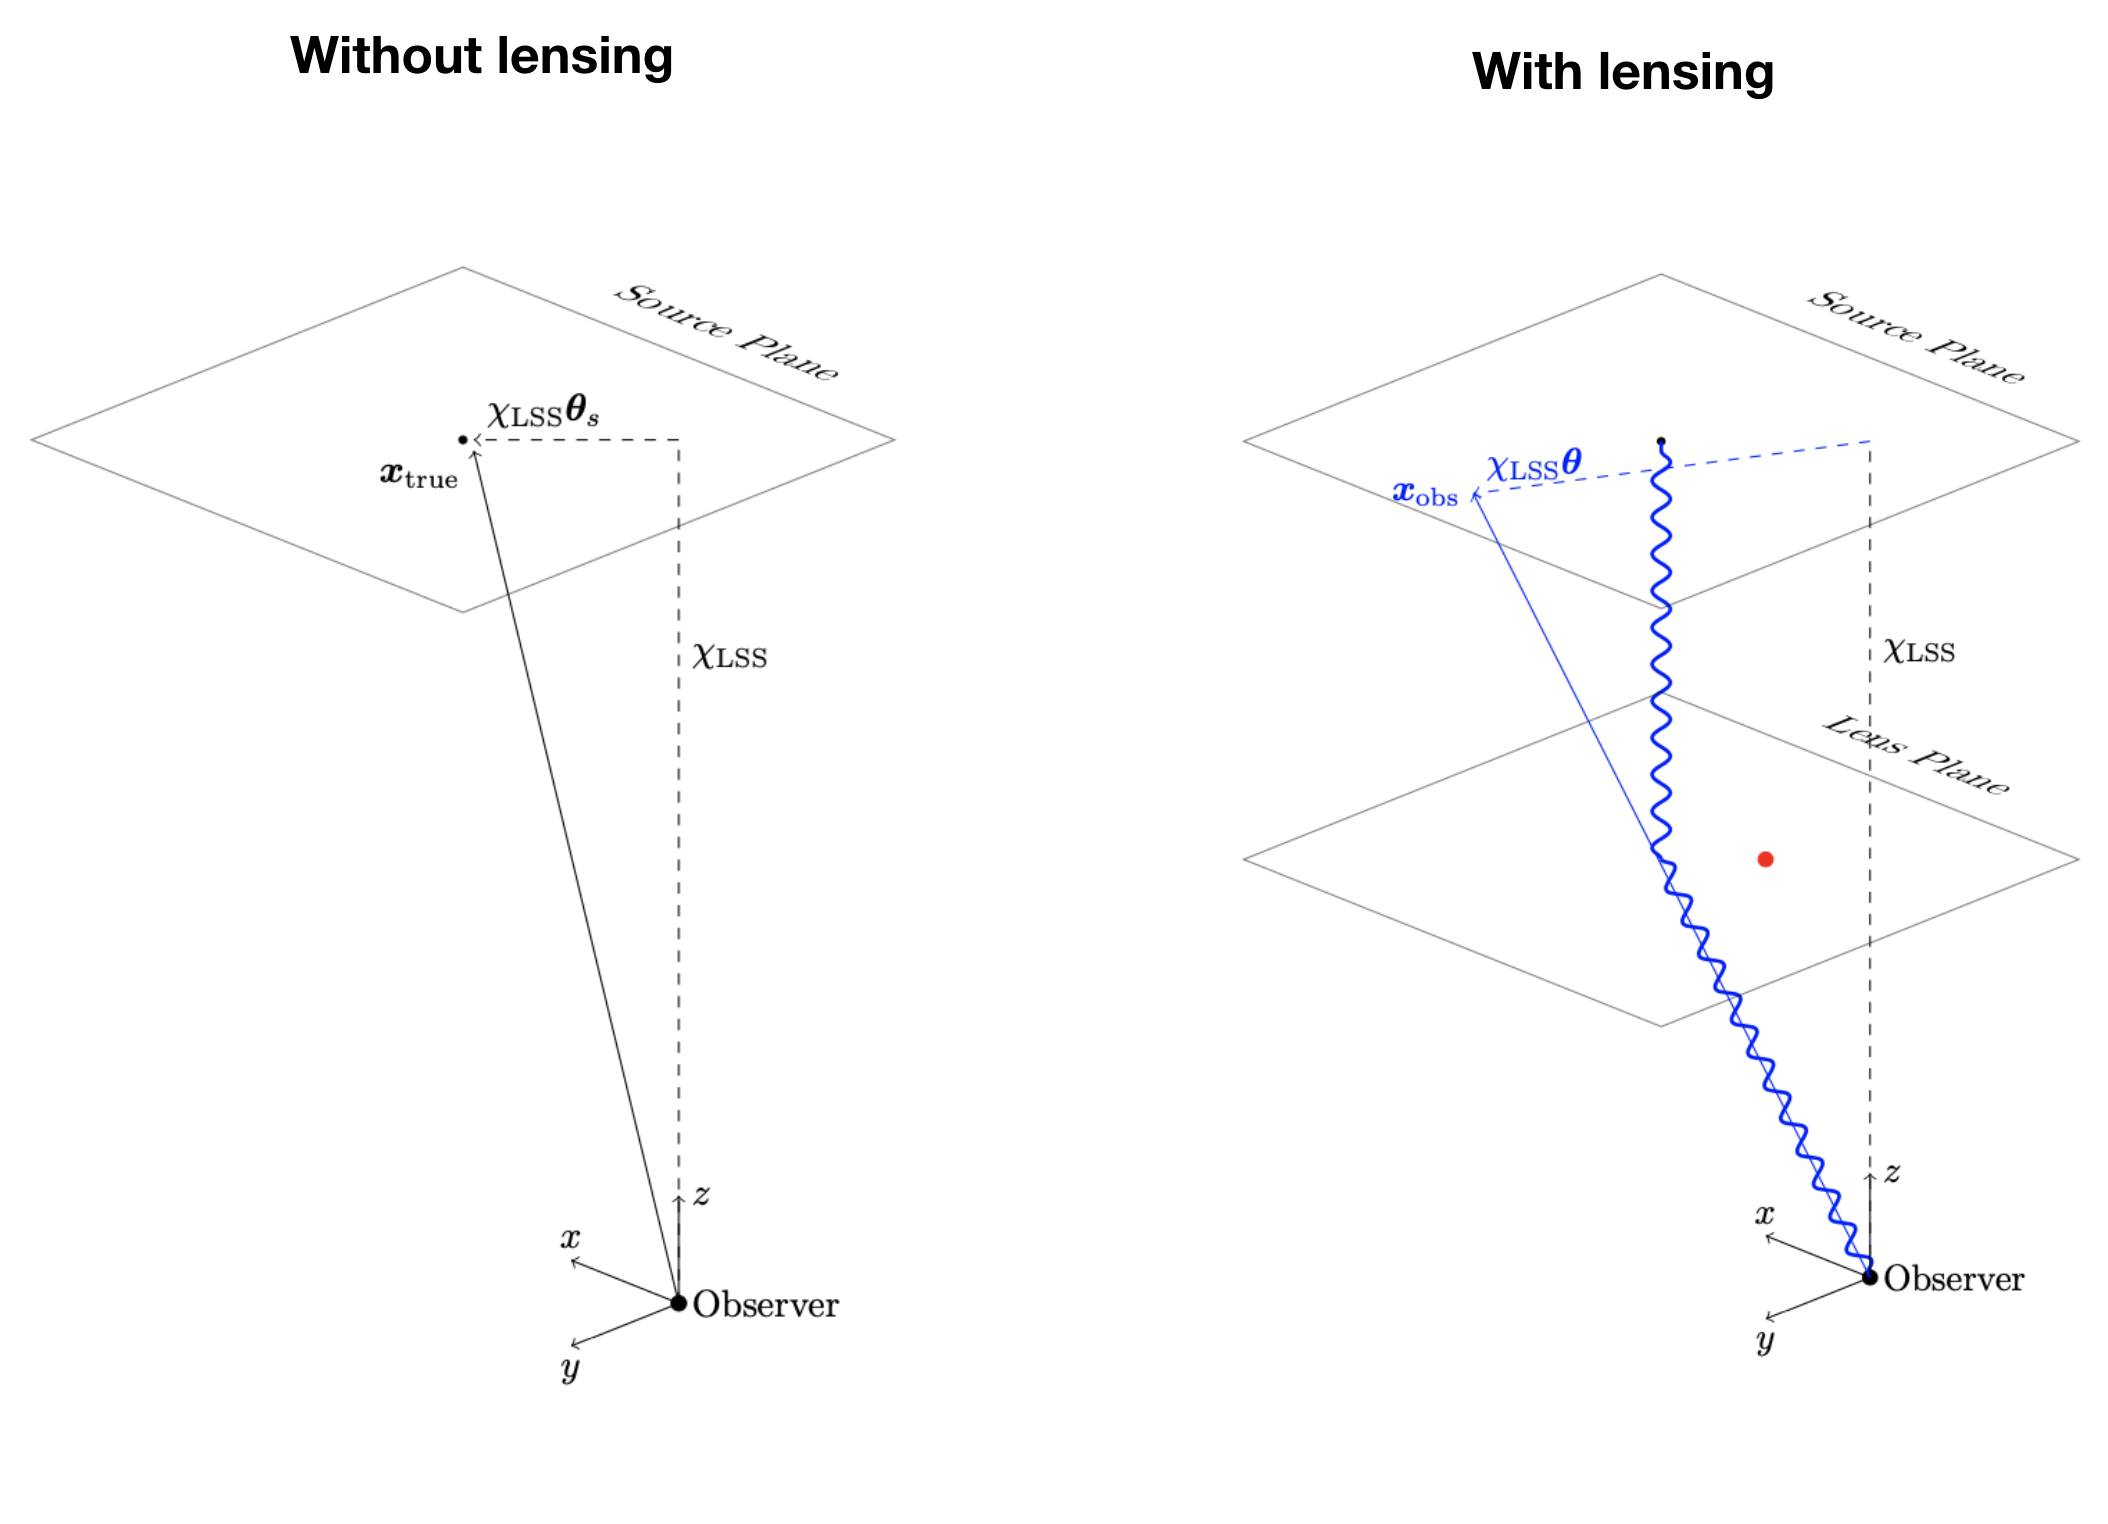
\includegraphics[width=0.7\columnwidth]{lensing.png}
  \caption{Path of a light ray without (left) and with (right) lensing.}
  \label{fig:lensing}
\end{figure}

\begin{figure}
\centering
\begin{tikzpicture}
% draw horizontal line
\draw (-4,0) -- (2,0);
% draw first vertical line
\draw (-1,-3) -- (-1,3) node[above] {lens plane};
% draw second vertical line
\draw (2,-3) -- (2,3) node[above] {source plane};

\draw[dashed] (-4,0) -- (2,1) node[right] {};

% draw intersection points
\filldraw (-1,0) circle (2pt) node[below right]{$x_{L}$};
\filldraw (2,1) circle (2pt) node[ right]{$x_{S} = x_{L}+ \delta x$};
\draw[->] (-2.5,0) arc[start angle=0, end angle=28, radius=0.5cm];
\node at (-2.8,0.5) {$\theta_{S}$};
\end{tikzpicture}
\caption{drawing for question (a)}
\label{fig:1dlensing}
\end{figure}


The lensing can be described from a remapping of the CMB photons from a position  
\ba
\bm{x}_{\rm true}  =\chi_{\rm LSS} \begin{pmatrix} 
{\theta}^{1}_{S} \cr
{\theta}^{2}_{S} \cr
 1
 \end{pmatrix} 
\ea
to a position 
\ba
\bm{x}_{\rm obs} = \chi_{\rm LSS}  \begin{pmatrix} 
{\theta}^{1} \cr
{\theta}^{2} \cr
 1
 \end{pmatrix} 
\ea
Where $\theta^{1}_{S}, \theta^{2}_{S}$ refers to the true source position, while  $\theta^{1}, \theta^{2}$ refers to its observed position (see Fig \ref{fig:lensing}).
$\chi_{\rm LSS}$ is the comoving distance to the last scattering surface. After a lengthy derivation (see paragraph 2 of \href{https://github.com/thibautlouis/thibautlouis.github.io/blob/master/derivation.pdf}{notes}), The relationship between the two position is given by
\ba
 \theta^{i}_{S}  &=&   \theta^{i} + \Delta  \theta^{i} \\
\ea
\ba
 \Delta  \theta^{i} &=& \delta^{ij} \frac{\partial }{\partial \theta^{j}} \phi^{L}(\bm{\theta}) \\
  \phi^{L}(\bm{\theta}) &=&  -2 \int^{\chi_{\rm LSS}}_{0} \frac{d\chi_{1}}{\chi_{1}}  \psi \left( \bm{x}(\bm{\theta}, \chi_{1}), \eta_{0}-\chi_{1} \right)  \left(1 - \frac{\chi_{1}}{\chi_{\rm LSS} } \right)
\ea
$  \phi^{L}(\bm{\theta}) $ is the lensing potential, its angular gradient will encode the change of position between true and observed position of the source.
We see that it is given as an integral along the line of sight of the gravitational potential $\psi$ times a geometric factor $ \left( \frac{\chi_{\rm LSS} -\chi_{1}}{\chi_{1}\chi_{\rm LSS} } \right)$ that account for where the deflection happens.
\begin{enumerate}
  \renewcommand{\labelenumi}{(\alph{enumi})}
\item (Optional) Let's check that the deflection has the correct sign, for simplicity let's think about it with a single lens and only two dimensions. The situation is represented in Figure \ref{fig:1dlensing}.
Let's imagine that the center of the lens sit at $x_{L}$, what will be the sign of $\Delta  \theta =  \theta_{S}  - \theta$ for a source located at $x_{S}= x_{L} + \delta x$ with $\delta x$ positive) ?

Tip: you can use that for $x>x_{L}$ on the lens plane,   $\frac{\partial }{\partial \theta} \psi  >0$ since $\psi$ is negative for over-density, and $\psi_{\rm min} = \psi(x_{L})$


\end{enumerate}

The lensing power is given by   (see paragraph 3 of \href{https://github.com/thibautlouis/thibautlouis.github.io/blob/master/derivation.pdf}{notes})
\ba
C^{L}_{\ell} =  4  \int^{\chi_{\rm LSS}}_{0}  d\chi_{1}  \left(\frac{\chi_{\rm LSS} - \chi_{1}}{\chi^{2}_{1}\chi_{\rm LSS} } \right)^{2}  P_{\psi} \left(k = \frac{\ell + 1/2}{\chi_{1}}, z(\chi_{1}) \right) 
\ea
This is the quantity we want to compute in this tutorial, we already have a way to compute $\chi$ so what we need is an expression for $P_{\psi} \left(k = \frac{\ell + 1/2}{\chi_{1}}, z(\chi_{1}) \right) $.
In order to get this expression, we need to solve the Einstein-Boltzmann equations for perturbation in the Universe, I have done it for you using the public code CAMB




\begin{enumerate}
\item First download the tar file at the following \href{https://github.com/thibautlouis/TD_ED_Phoeenix/blob/main/data.tar.gz}{url}, and untar it, the data consist of a power spectrum of the form $k^{2}P_{\psi}(k,z)$ for different value of k and z.
We will make an interpolation table using the following function  \\ \\
 \begin{lstlisting}[language=Python]
import numpy as np
from scipy.interpolate import interp2d

def get_P_z_and_k_interp(mode):
    """
    This function read and interpolate k^{2}P_{\psi}(k,z)
    
    Parameters
     ----------
    H0: float
        Hubble constant value in km/s/Mpc

    """

    P_z_and_k = np.load(f"data/P_k_and_z_{mode}.npy")
    k_array = np.load("data/k_array.npy")
    z_array = np.load("data/z_array.npy")
    P_z_and_k_interp = interp2d(z_array, k_array, P_z_and_k.flatten())
    return z_array, k_array, P_z_and_k_interp

\end{lstlisting}
I have precomputed $k^{4}P_{\psi}(k,z)$   for two modes, 'lcdm' and 'baryons\_only', we will first do the computation with the lcdm mode.
\item Plot $k^{4}P_{\psi}$  as a function of k at different redshift $z = [0, 0.5, 1, 4 ,20]$
\item   The integral from $C^{L}_{\ell} $ goes from 0 to the comoving distance to the last scattering surface $\chi_{\rm LSS}$, you can see that it diverges at 0, in reality this doesn't affect the result because it only affect the $\ell =0$ term. However it can lead to numerical instability so instead of doing the integral  $\int^{\chi_{\rm LSS}}_{0}  d\chi_{1}$ we will do $\int^{\chi_{\rm LSS}}_{\chi_{\rm min}}  d\chi_{1}$ with $\chi_{\rm min}=10$.

Create an evenly spaced array $\chi$ of comoving distance between $\chi_{\rm min}$ and $\chi_{\rm LSS}$ containing 100 values.
\item Create an array of the corresponding redshift values $z(\chi)$ using the interpolation function that we have defined in Section 2.
\item Ok time to do the integral, we will compute the lensing power spectrum for $\ell \in [2, 2000]$, looking at the formula we see that the lensing potential will be computed as  \\ \\

 \begin{lstlisting}[language=Python]
l_array = np.arange(2, 2000 + 1, dtype=np.float64)
cl_phi = np.zeros(l_array.shape)
for i, l in enumerate(l_array):
    k_array = (l + 0.5) / chi_array
    cl_phi[i] = 0
    for z, chi, k in zip(z_array, chi_array, k_array):
        cl_phi[i] += 4 * dchis * P_z_and_k_interp(z, k) * ((chi_star - chi) / (chi ** 2 * chi_star)) ** 2 / k ** 4
\end{lstlisting}

Plot the resulting $\ell^\frac{5}{2}(\ell+1)^{2} C_{\ell}^{L}$ and compare it with Figure 1.

\item In the same tarball as for question 1, you will find the measured lensing power spectrum "result\_act.dat" with format, $\ell_{b}, \ell_{b}^\frac{5}{2}(\ell_{b}+1)^{2} C_{\ell_{b}}^{L}, \ell_{b}^\frac{5}{2}(\ell_{b}+1)^{2} \sigma_{\ell_{b}}^{L}$, where $\sigma$ are the errors on the measurement and $\ell_{b}$ the central value of the $\ell$ bin. Plot these data on the top of the theory curve. Note that there are small deviations compared to Figure 1, this is due to some approximations we made along the way in this derivation.
\item Redo the computation for the mode  'baryons\_only', and conclude.





\end{enumerate}

%Let's define $x^{i}_{\perp}= \chi \theta_{S}^{i}$, we know of the evolution equation for $\bm{x}$, this is 
%\ba
%\frac{dx^{i}}{dt} = \frac{P^{i}}{P^{0}} = \frac{\hat{p}^{i}}{a}\frac{p}{E}(1 - \phi + \psi)
%\ea
%for light ray we have 
%\ba
%ds^{2} =  a^{2}(\eta) [ (1 + 2\psi)d\eta^{2} - ( 1- 2\phi)\delta_{ij}d\chi^{2}] = 0 \\
%d\eta = -d\chi
%\ea

\end{document}



